% !TeX root = ../main.tex
% Add the above to each chapter to make compiling the PDF easier in some editors.

\chapter{Software Application}\label{Software Application}

\section{Application Structure}
The software application is basically an android application composed of two layers: the native layer, written in C++ and the Java layer. 
The Java layer includes user interface (UI) components of the application and all application business logic. 
The C++ layer is responsible for communicating with the camera as well as for image processing of raw images coming from the camera using open computer vision library (OpenCV).

Because compiled Java code runs on the Java virtual machine (JVM) which is a part of the Java runtime environment (JRE). Whereas compiled C++ runs directly on the operating system (OS), a bridging component Between the two layers is needed.
The Java native interface (JNI) allows the two layers to interact with each other. It is a Java feature that allows Java code to call native applications and libraries written in languages such as C, C++ and Objective-C.

The \autoref{fig:applicationArchitecture} below shows the application high-level architecture.


\begin{figure}[H]
\centering
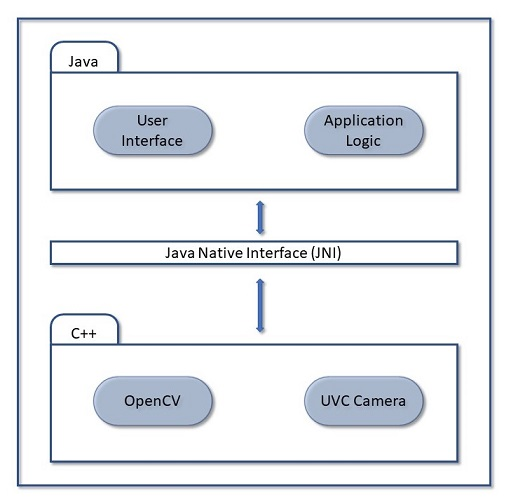
\includegraphics{figures/applicationArchitecture.JPG}
\caption[Application architecture]{Application architecture}\label{fig:applicationArchitecture}
\end{figure}


\subsection{C++ Layer}
\subsubsection{USB Video Class}

USB Video Class (UVC) describes the capabilities and characteristics of video streaming devices. It is widely used, such as desktop video cameras (or "webcams"), digital camcorders, still-image cameras, and so forth. USB Video Class (UVC) is a standard class specification that standardizes video streaming functionality on the USB. It enables devices like webcams, digital camcorders, analog video converters, analog and digital television tuners etc to connect seamlessly with host machines. UVC supports streaming multiple video formats including and provides structures for describing the functionalities of the video device to the host and defines USB requests to control different parameters of the device and characteristics of the video stream. It also provides flexibility for a video device to support multiple video resolutions, formats and frame rates, which highly influences the bandwidth negotiation between the device and the host \parencite{uvc}.

\subsubsection{UVC Camera Library for Android}
Many OS platforms have native support for UVC drivers which greatly reduces the time required for developers to connect UVC devices. Unfortunately, android doesn’t offer such a support, therefore, to connect a UVC device such as a webcam, the device driver must be written by the developer. 
Nevertheless, third-party and open source libraries offer good alternative solution for the UVC device drivers. An open source library to access to UVC webcams on non-rooted Android device called UVCCamera was used in this project \parencite{uvcCamera}. The library works on minimum android version 3.1 or later (API >= 12), but Android 4.0(API >= 14) or later is recommended.



\subsection{Java Layer}


The compiled Java code along with any data and resource files required by the application is bundled by the android asset packaging tool (AAPT) tool into an android package, an archive file marked by an .apk suffix.
The Java layer includes the user interface (UI) components and all application buisness logic.

\subsection{Permissions}
\subsubsection{USB Host}
By default, Android does not allow an application to access the devices connected to the OTG  port. To enable an application to interact with a the UVC camera directly connected on an OTG port, a few additional steps are required.

 In \texttt{AndroidManifest.xml}, the "USB Host" functionality must be declared by adding the \texttt{<uses-feature android:name="android.hardware.usb.host"/>} tag in the manifest section.

\subsubsection{Open GL}

\subsubsection{User Interface}

\subsubsection{Image Processing}

\subsection{Native C++ Layer}
